\documentclass[12pt]{article}
\usepackage[margin=1in]{geometry}
\usepackage[utf8]{inputenc}
\usepackage[spanish]{babel}
\usepackage{parskip}
\usepackage{setspace}
\usepackage{amsmath}
\usepackage{graphicx}
\usepackage{tikz}
\usepackage{hyperref}

% Opciones de paquetes.
\decimalpoint % {babel}
\onehalfspacing % {setspace}
\graphicspath{{./img/}} % {graphicx}
\usetikzlibrary{babel} % Para que tikz no conflictue con {babel} con figuras como "->".

% Encabezado
\title{Clase 32. Curvas Paramétricas.}
\author{MIT 18.01: Single Variable Calculus.}
\date{}

\begin{document}
\maketitle

\begin{abstract}
\noindent En esta y la siguiente clase veremos dos usos de la fórmula de la longitud de arco. La primera será en curvas paramétricas, que son aquellas formadas por la trayectoria de un punto que está en función de una tercera variable. Estudiaremos en qué consisten, así como revisaremos ejemplos para calcular sus arcos y áreas de superficies de revolución.
\end{abstract}


\section{Curvas Paramétricas.}

A lo largo del curso hemos trabajado con curvas que pueden ser expresadas como una función $y = f(x)$. Sin embargo, muchas veces esto no es posible porque en algunas de ellas su valor de entrada $x$ resulta en más de un valor de salida $y$, incumpliéndose la condición para que pueda ser catalogada como función\footnote{A nivel geométrico, nos estamos refiriendo a que se falla en la prueba de la recta vertical.}.

A pesar de que no siempre es posible expresar a una curva como función, en ocasiones sí se puede con sus \textbf{coordenadas}, las cuales podemos escribir en términos de una \textbf{nueva variable} llamada \textbf{parámetro}. A éstas se las conoce como \textbf{Curvas Paramétricas}.

Así, toda curva cuyas coordenadas $(x, \ y)$ pueden ser expresadas como
\begin{align*}
  x &= g(t) &  y &= h(t)
\end{align*}
recibe el nombre de curva paramétrica, donde $t$ es su parámetro, mientras que $g(t)$ y $h(t)$ se conocen como las \textbf{ecuaciones paramétricas} de la curva.

Un ejemplo de una curva paramétrica es la trayectoria que va dejando una partícula al estar en movimiento, donde son sus coordenadas las que varían en función del tiempo $t$.

\newpage

\begin{figure}[hbt!]
\centering
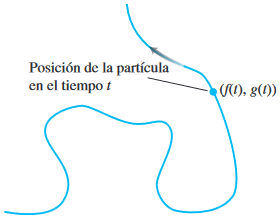
\includegraphics[scale=0.55]{curva-parametrica.jpg}
\caption{Thomas, G (2010). \textit{Cálculo. Una Variable}. Pp. 610.}
\end{figure}


\section{Longitud de Arco y Tasa de Cambio en una Curva Paramétrica.}

La clase anterior aprendimos a calcular la longitud de arco de una curva. Llevemos este conocimiento a aquellas que son paramétricas.

Sea $C$ una curva continua y derivable que es definida por las siguientes ecuaciones paramétricas, donde $a \leq t \leq b$:
\begin{align*}
  x &= f(t) & y &= g(t)
\end{align*}
Además, supongamos que $f(t)$ y $g(t)$ son derivables en $[a, \ b]$.

Dividamos la curva $C$ en $n$ subintervalos todos de ancho $\Delta t$, donde cada punto corresponde a la coordenada $P_{i}(x_{i}, \ y_{i}) = P_{i}(f(t_{i}), \ g(t_{i}))$, para $i = 1, \ 2, \ \cdots, \ n$. Luego, unámoslos mediante segmentos de rectas para formar la trayectoria poligonal.

\begin{figure}[hbt!]
\centering
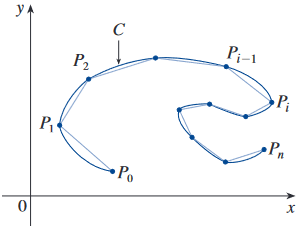
\includegraphics[scale=0.5]{longitud-de-curva-parametrica.jpg}
\caption{Stewart, J (2017). \textit{Cálculo. Trascendentes Tempranas}. Pp. 652.}
\end{figure}

De igual modo a como lo hicimos en la clase 31, para aproximarnos a la longitud de arco de $C$ sumemos cada segmento de la trayectoria poligonal, los cuales a su vez se acercan a cada subintervalo $s_{i}$ de la curva y que obtenemos al aplicar el Teorema de Pitágoras.
\[
  \Delta s_{i} \approx \sqrt{(\Delta x_{i})^{2} + (\Delta y_{i})^{2}} = \sqrt{(\Delta f(t_{i}))^{2} + (\Delta g(t_{i}))^{2}}
\]
Debido a que $f(t)$ y $g(t)$ son continuas y derivables en $[a, \ b]$, por el Teorema del Valor Medio podemos establecer que:
\begin{align*}
  \frac{\Delta f(t)}{\Delta t} &= \left. \frac{df}{dt} \right|_{t = c} & \frac{\Delta g(t)}{\Delta t} &= \left. \frac{dg}{dt} \right|_{t = d}
\end{align*}
con $a < c < b$ y $a < d < b$.

Reordenemos las ecuaciones obtenidas por el Teorema del Valor Medio.
\begin{align*}
  \Delta f(t) &= \left. \frac{df}{dt} \right|_{t = c} \cdot \Delta t & \Delta g(t) &= \left. \frac{dg}{dt} \right|_{t = d} \cdot \Delta t
\end{align*}
Puesto que $x = f(t)$ e $y = g(t)$, entonces
\begin{align*}
  \Delta x &= \left. \frac{dx}{dt} \right|_{t = c} \cdot \Delta t & \Delta y &= \left. \frac{dy}{dt} \right|_{t = d} \cdot \Delta t
\end{align*}
Así:
\[
  \Delta s_{i} \approx \sqrt{
                              \left(\left. \frac{dx_{i}}{dt} \right|_{t = c} \Delta t\right)^{2} +
                              \left(\left. \frac{dy_{i}}{dt} \right|_{t = d} \Delta t\right)^{2}
                            }
               = \sqrt{\left(\left. \frac{dx_{i}}{dt} \right|_{t = c} \right)^{2} + \left(\left. \frac{dy_{i}}{dt} \right|_{t = d} \right)^{2}}
                 \Delta t
\]
La suma de los subintervalos $\Delta s_{i}$ a medida que $n \to \infty$ corresponde a la \textbf{longitud de arco de una curva paramétrica} $C$, la cual denotaremos como $L$.
\[
  L = \lim_{n \to \infty}
       \sum_{i = 1}^{n} \sqrt{\left(\left. \frac{dx_{i}}{dt} \right|_{t = c} \right)^{2} + \left(\left. \frac{dy_{i}}{dt} \right|_{t = d} \right)^{2}}
       \Delta t
    = \int_{t = a}^{t = b} \sqrt{\left(\frac{dx}{dt}\right)^{2} + \left(\frac{dy}{dt}\right)^{2}} dt
\]
Ahora digamos que $ds$ es un segmento infinitesimal de la curva $C$. En ese contexto, podemos calcular su medida como:
\[
  ds = \sqrt{\left(\frac{dx}{dt}\right)^{2} + \left(\frac{dy}{dt}\right)^{2}} dt
\]
Si la multiplicamos por $(1/dt)$ obtenemos la \textbf{tasa de cambio instantánea} del punto $(x, \ y) = (f(t), \ g(t))$ que genera la curva $C$.

\[
  \frac{ds}{dt} = \sqrt{\left(\frac{dx}{dt}\right)^{2} + \left(\frac{dy}{dt}\right)^{2}}
\]
En física, $ds/dt$ corresponde a la \textbf{rapidez} con que se mueve la particula $(x, \ y)$.

\textbf{Ejemplo 1.} Encuentre la curva, la dirección de su movimiento, la longitud de arco y la tasa de cambio de las ecuaciones paramétricas:
\begin{align*}
  x &= a \ \cos(t) & y &= a \ \sin(t); \ (a = \text{constante})
\end{align*}
\textbf{Solución.} Sin necesidad de crear una tabla de valores para $x$ e $y$, podemos elevar ambas variables al cuadrado y sumarlas para conocer rápidamente su curva.
\[
  x^{2} + y^{2} = (a \cos(t))^{2} + (a \sin(t))^{2} = a^{2} \cos^{2}(t) + a^{2} \sin^{2}(t) = a^{2}(\cos^{2}(t) + \sin^{2}(t)) = a^{2}
\]
En otras palabras, las ecuaciones paramétricas $x = a \cos(t)$ e $y = a \sin(t)$ forman la curva de un círculo $x^{2} + y^{2} = a^{2}$ con radio $r = a$.

Para conocer la dirección en que se mueve el punto $(x = a \cos(t), \ y = a \sin(t))$ démosle valores a $t$ y observemos sus valores de salida.

\begin{table}[hbt!]
\centering

\begin{tabular}{c|c c c}
$t$ & $0$ & $\pi / 2$ & $\pi$ \\
\hline
$(x, \ y)$ & $(a, \ 0)$ & $(0, \ a)$ & $(-a, \ 0)$
\end{tabular}

\end{table}

Como vemos en la tabla, a medida $t$ toma valores mayores o iguales a cero, el punto $(x, \ y)$ va desplazándose a \textbf{contrarreloj} a lo largo de la circunferencia de $x^{2} + y^{2} = a^{2}$.

\begin{figure}[hbt!]
\centering

\begin{tikzpicture}
%\draw[help lines] (-8, -3) grid (8, 3);

% Ejes.
\draw[<->, line width=0.3mm] (-3, 0) -- (3, 0) node [right] {$x$};
\draw[<->, line width=0.3mm] (0, -3) -- (0, 3) node [left] {$y$};

% Círculo paramétrico (red!60 = 60% de rojo).
\draw [->, line width=0.6mm, color = red!60] (2, 0) arc (0:88:2cm);
\draw [->, line width=0.6mm, color = red!60] (0, 2) arc (90:178:2cm);
\draw [->, line width=0.6mm, color = red!60, dashed] (-2, 0) arc (180:358:2cm);

% Puntos
\draw[fill = blue, color = blue] (2, 0) circle (0.7mm);
\draw[fill = blue, color = blue] (0, 2) circle (0.7mm);
\draw[fill = blue, color = blue] (-2, 0) circle (0.7mm);


% Etiquetas.
\node at (2.6, -0.4) {$(a, \ 0)$};
\node at (-0.6, 2.3) {$(0, \ a)$};
\node at (-2.7, -0.4) {$(-a, \ 0)$};

\node at (2.5, 0.4) {$t = 0$};
\node at (1, 2.3) {$t = \frac{\pi}{2}$};
\node at (-2.65, 0.4) {$t = \pi$};
\end{tikzpicture}

\end{figure}

Como la curva de las ecuaciones paramétricas $x = a \cos(t)$ e $y = a \sin(t)$ forman un círculo, calcularemos su longitud de arco en el intervalo $0 \leq t \leq 2\pi$.
\[
  \int_{0}^{2\pi} \sqrt{\left(-a \sin(t)\right)^{2} + \left(a \cos(t)\right)^{2}} dt =
    \int_{0}^{2\pi} \sqrt{a^{2} \left(\sin^{2}(t) + \cos^{2}(t)\right)} dt =
    \int_{0}^{2\pi} a dt =
    2\pi a
\]
A partir de la longitud de arco del círculo de radio $a$ podemos calcular la tasa en la que se mueve el punto $(a \cos(t), \ a \sin(t))$.
\[
  \frac{ds}{dt} = \sqrt{a^{2} \sin^{2}(t) + a^{2} \cos^{2}(t)} = a
\]
Es decir, el punto $(a \cos(t), \ a \sin(t))$ se mueve a una rapidez uniforme de $a$.

\textbf{Ejemplo 2.} Calcule la forma, dirección de movimiento y longitud de la curva generada por las ecuaciones paramétricas
\begin{align*}
  x &= 2 \sin(t) & y = \cos(t)
\end{align*}
\textbf{Solución.} Al igual que en el ejemplo anterior, podemos sumar el cuadrado de $x$ y el cuadrado de $y$, pero debido al número $2$ que multiplica a la primera variable, tendremos que multiplicarla por $(1/4)$ para deshacernos de éste.
\[
  \frac{1}{4} x^{2} + y^{2} = \frac{1}{4} (2 \sin(t))^{2} + \cos^{2}(t) = 1
\]
Por lo tanto, las ecuaciones paramétricas $x = 2 \sin(t)$ e $y = \cos(t)$ forman una \textbf{elipse unitaria} (i.e, de radio $r = 1$) dada por la ecuación $(1/4) x^{2} + y^{2} = 1$.

Luego, démosle valores a $t \geq 0$ para ver en qué dirección se mueve el punto $(2 \sin(t), \ \cos(t))$.

\begin{table}[hbt!]
\centering

\begin{tabular}{c|c c c}
$t$ & $0$ & $\pi / 2$ & $\pi$ \\
\hline
$(x, \ y)$ & $(0, \ 1)$  & $(2, \ 0)$  & $(0, \ -1)$
\end{tabular}

\end{table}

Como vemos a continuación, $(2 \sin(t), \ \cos(t))$ se mueve en dirección de las agujas del reloj.

\begin{figure}[hbt!]
\centering

\begin{tikzpicture}
% Help lines
%\draw [help lines] (-8, -3) grid (8, 3);

% Ejes.
\draw [<->, line width = 0.3mm] (-3, 0) -- (3, 0) node [right] {$x$};
\draw [<->, line width = 0.3mm] (0, -2) -- (0, 2) node [left] {$y$};

% Elipse paramétrica.
\draw [->, line width = 0.6mm, color = red!60] (0, 1) arc [start angle = 90, end angle = 4, x radius = 2cm, y radius = 1cm];
\draw [->, line width = 0.6mm, color = red!60] (2, 0) arc [start angle = 0, end angle = -88, x radius = 2cm, y radius = 1cm];
\draw [->, line width = 0.6mm, dashed, color = red!60] (0, -1) arc [start angle = -90, end angle = -266, x radius = 2cm, y radius = 1cm];

% Puntos.
\draw [fill = blue, color = blue] (0, 1) circle (0.7mm);
\draw [fill = blue, color = blue] (2, 0) circle (0.7mm);
\draw [fill = blue, color = blue] (0, -1) circle (0.7mm);

% Etiquetas.
\node at (-0.2, -0.2) {$0$}; % Origen
\node at (-0.6, 1.35) {$t = 0$};
\node at (0.6, 1.35) {$(0, \ 1)$};
\node at (2.75, 0.4) {$t = \pi / 2$};
\node at (2.6, -0.4) {$(2, \ 0)$};
\node at (0.6, -1.35) {$t = \pi$};
\node at (-0.75, -1.35) {$(0, \ -1)$};
\end{tikzpicture}

\end{figure}

Finalmente, calculemos la longitud de la curva completa generada por $x = 2 \sin(t)$ e $y = \cos(t)$ en $0 \leq t \leq 2\pi$.
\[
  \int_{0}^{2\pi} \sqrt{4\sin^{2}(t) + \cos^{2}(t)} dt
\]
Debido a que la integral de arriba no es elemental (i.e, no podemos resolverla de forma analítica), dejamos expresada de esa manera a la longitud de la curva paramétrica de este ejemplo.


\section{Área de Superficie de una Curva Paramétrica.}

La clase pasada vimos que, con la ayuda de la fórmula de la longitud de arco, podemos calcular el área de una superficie de revolución como:
\begin{align*}
  (1) \ \int_{a}^{b} 2 \pi y \cdot ds &= \int_{a}^{b} 2 \pi y \cdot \sqrt{1 + \left(\frac{dy}{dx}\right)^{2}} dx \\
  (2) \ \int_{a}^{b} 2 \pi x \cdot ds &= \int_{a}^{b} 2 \pi x \cdot \sqrt{1 + \left(\frac{dx}{dy}\right)^{2}} dy
\end{align*}
Cuando la superficie es generada al rotar una \textbf{curva paramétrica}, la fórmula de su área es similar, pero debe estar en términos del parámetro $t$ puesto que $x$ e $y$ están en función de él.
\begin{align*}
  (3) \ \int_{t = a}^{t = b} 2 \pi y(t) \cdot ds &=
    \int_{t = a}^{t = b} 2 \pi y(t) \cdot \sqrt{\left(\frac{dx}{dt}\right)^{2} + \left(\frac{dy}{dt}\right)^{2}} dt \\
  (4) \ \int_{t = a}^{t = b} 2 \pi x(t) \cdot ds &=
    \int_{t = a}^{t = b} 2 \pi x(t) \cdot \sqrt{\left(\frac{dx}{dt}\right)^{2} + \left(\frac{dy}{dt}\right)^{2}} dt
\end{align*}
Para evitar posibles confusiones, en las fórmulas $(3)$ y $(4)$ debemos tener en cuenta que:

\begin{itemize}
\item Ecuación $(3) \rightarrow$ Área de Superficie con respecto a $x$.
\item Ecuación $(4) \rightarrow$ Área de Superficie con respecto a $y$.
\end{itemize}

\textbf{Ejemplo 3.} Calcule el área de la superficie de una elipsoide generada al hacer rotar una elipse alrededor del eje $y$ que proviene de las ecuaciones paramétricas:
\begin{align*}
  x &= 2 \sin(t) & y = \cos(t)
\end{align*}
\textbf{Solución.} Las ecuaciones paramétricas de la elipse son las mismas del ejemplo anterior, lo que implica que
\[
  ds = \sqrt{4\sin^{2}(t) + \cos^{2}(t)} dt
\]
Como la elipsoide es generada al hacer girar a la elipse con respecto al eje $y$, para calcular su área de superficie usamos la ecuación $(3)$ y debido a que solo necesitamos una mitad de esta figura para obtener al sólido, evaluaremos a la integral en el intervalo\footnote{Podemos revisar la figura de la elipse del Ejemplo 2 para comprobar que es el intervalo correcto.} $0 \leq t \leq \pi$.
\[
  \int_{0}^{\pi} 2\pi (2 \sin(t)) \cdot \sqrt{4\sin^{2}(t) + \cos^{2}(t)} dt
\]
A diferencia del ejemplo 2, esta integral puede ser calculada, pero debido a que el proceso es muy largo, la dejaremos tal como está arriba.
\end{document}
